% === [ Introduction ] =========================================================

% ====>>>>> Primer

% Fuzzy Graph Theory

% Quickly cover the background terminology of Fuzzy Logic and Fuzzy Graph
% Theory.

\begin{frame}
	\frametitle{A Primer to Fuzzy Graph Theory}

	% Fuzzy Logic used to handle uncertainty.
	\begin{enumerate}
		\item Fuzzy Logic
		\item Fuzzy Graph Theory
	\end{enumerate}
\end{frame}

\begin{frame}
	\frametitle{Fuzzy Logic}

	Definitions from ``Fuzzy graphs'' {\footnotesize (Rosenfeld, 1975)}.

	\begin{block}{Fuzzy subsets}
		% sigma
		\textbf{Definition}: A \textit{fuzzy subset} of a set $S$ is a mapping $\sigma: S \rightarrow [0, 1]$ which assigns each element $x \in S$ a degree of membership $0 \le \sigma(x) \le 1$.

		\vspace*{2em}

		\textbf{Examples}:
		\begin{itemize}
			\item $Deina \in old$ with $\sigma(Deina) = 0.3$
			\begin{itemize}
				\item The element $Deina$ (woman at age $34$) is a member of the set $old$ to a degree of $0.3$
			\end{itemize}
			\item $Foufoutos \in old$ with $\sigma(Foufoutos) = 0.5$
			\begin{itemize}
				\item The element $Foufoutos$ (man at age $45$) is a member of the set $old$ to a degree of $0.5$
			\end{itemize}
			\item $Tade \in old$ with $\sigma(Tade) = 0.1$
			\begin{itemize}
				\item The element $Tade$ (boy at age $6$) is a member of the set $old$ to a degree of $0.1$
			\end{itemize}
		\end{itemize}
	\end{block}
\end{frame}

% contributions:
% * show how to generalize fuzzy relation to map into a fuzzy subset of a set $S$.
% * present fuzzy analogs of graph-theoretic concepts.

\begin{frame}
	\frametitle{Fuzzy Logic}

	\begin{block}{Fuzzy relations}
		% mu
		\textbf{Definition}: A \textit{fuzzy relation} on a set $S$ is a mapping $\mu: S \times S \rightarrow [0, 1]$ which assigns each ordered pair $(x, y) \in S \times S$ a degree of membership $0 \le \mu(x, y) \le 1$. In other words, a fuzzy relatipship on $S$ is a fuzzy subset of $S \times S$.

		\vspace*{2em}

		\textbf{Examples}:
		\begin{itemize}
			\item $(Deina, Tade) \in mothers$ with $\mu(Deina, Tade) = 1.0$, where $mothers: person \times person$
			\begin{itemize}
				\item The ordered pair $(Deina, Tade)$ is a $(mother, child)$-relation on the set $person$ to a degree of $1.0$
			\end{itemize}
			\item $(Foufoutos, Tade) \in fathers$ with $\mu(Foufoutos, Tade) = 0.5$, where $fathers: person \times person$
			\begin{itemize}
				\item The ordered pair $(Foufoutos, Tade)$ is a $(father, child)$-relation on the set $person$ to a degree of $0.5$
			\end{itemize}
		\end{itemize}
	\end{block}
\end{frame}

\begin{frame}
	\frametitle{Fuzzy Logic}

	Definitions from ``Fuzzy morphisms between graphs'' {\footnotesize (Perchant \& Bloch, 2002)}.

	\begin{block}{Fuzzy relation on $\sigma_1 \times \sigma_2$}
		Let $\sigma_1: S_1 \rightarrow [0, 1]$ and $\sigma_2: S_2 \rightarrow [0, 1]$ be fuzzy subsets of $S_1$ and $S_2$, respectively. \\
		\textbf{Definition}: The function $\mu: S_1 \times S_2 \rightarrow [0, 1]$ is a \textit{fuzzy relation} on $\sigma_1 \times \sigma_2$ iff:

		\begin{equation}
			\begin{aligned}
				& \forall (x, y) \in S_1 \times S_2: \\
				& \mu(x, y) \le \sigma(x) \fuzzmin \sigma(y)
			\end{aligned}
			\label{eq:fuzzy_relation}
		\end{equation}

		{\small \textbf{Note}: $\fuzzmin$ denotes \textit{minimum} (and $\fuzzmax$ denotes \textit{maximum}).}

		\vspace*{2em}

		\textit{Intuition}: A fuzzy relation cannot be ``stronger'' than either of its elements.
	\end{block}
\end{frame}

\begin{frame}
	\frametitle{Fuzzy Graph Theory}

	\begin{block}{Fuzzy graph}
		\textbf{Definition}: A \textit{fuzzy graph} $F = (\sigma, \mu)$ is a pair of functions $\sigma: S \rightarrow [0, 1]$ and $\mu: S \times S \rightarrow [0, 1]$ which satisfy equation \ref{eq:fuzzy_relation} (of previous slide).

		\vspace*{2em}

		\textit{Intuition}: For a given graph $G(V, E)$, a fuzzy graph $F(\sigma, \mu)$ has a fuzzy subset $\sigma$ of $V$ and a fuzzy subset $\mu$ of $V \times V$. Since equation \ref{eq:fuzzy_relation} (of previous slide) is satisfied, a ``fuzzy edge'' cannot be stronger than either of its ``fuzzy endpoint verticies''.
	\end{block}
\end{frame}

\begin{frame}
	\frametitle{Fuzzy Graph Theory}

	\begin{block}{Max-min composition}
		Let $\mu_1$ and $\mu_2$ be two fuzzy relations on $\sigma_1 \times \sigma_2$ and $\sigma_2 \times \sigma_3$, respectively. \\
		\textbf{Definition} A \textit{max-min composition} of $\mu_1$ and $\mu_2$, denoted by $\mu_1 \maxmincomposition \mu_2$, is defined as follows.

		\begin{equation}
			\begin{aligned}
				& \forall (u_1, u_3) \in S_1 \times S_3, (u_1 \maxmincomposition u_2) (u_1, u_3) \\
				& = \sup_{u_2 \in S_2}\{ \mu_1(u_1, u_2) \fuzzmin \mu_2(u_2, u_3) \}
			\end{aligned}
			\label{eq:min_max_composition}
		\end{equation}

		% sup: smallest number great than or equal to all numbers in the set.
		\textbf{Note}: $\sup$ (supremum) denotes \textit{least upper bound} (and $\fuzzmin$ denotes \textit{minimum}).

		\vspace*{2em}

		\textit{Intuition}: select the best ``middle'' vertex $u_2$ such that a path from $u_1$ to $u_2$ and $u_2$ to $u_3$ has the highest ``quality'', as measured by the lowest edge weight $\mu(x, y)$ along that path.
	\end{block}
\end{frame}

\begin{frame}
	\frametitle{Fuzzy Graph Theory}

	\begin{block}{Max-min composition}

	Going through $u_2$ improves ``quality'' of path from $\mu(u_1, u_3) = 0.3$ to $(u_1 \maxmincomposition u_2)(u_1, u_3) = 0.5$.

	\begin{figure}[htbp]
		\centering
		\begin{subfigure}[t]{0.25\textwidth}
			\centering
			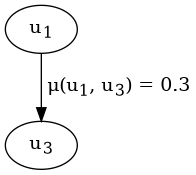
\includegraphics[width=\linewidth,valign=t]{inc/fuzzy_graph_theory/maxmincomposition_before.png}
			\caption{Path from $u_1$ to $u_3$.}
		\end{subfigure}
		\quad
		\begin{subfigure}[t]{0.25\textwidth}
			\centering
			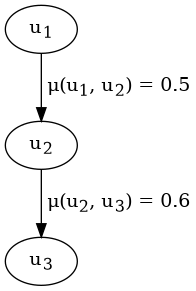
\includegraphics[width=\linewidth,valign=t]{inc/fuzzy_graph_theory/maxmincomposition_after.png}
			\caption{Path from $u_1$ through $u_2$ to $u_3$.}
		\end{subfigure}
		\caption{Find better ``quality'' path using max-min composition.}
	\end{figure}

	\end{block}
\end{frame}
